  \documentclass{article}
  \usepackage[utf8]{inputenc}

  % --- DOCUMENT LAYOUT & STYLING ---
  \usepackage{geometry} % Control page margins
  \usepackage{pgfgantt}
  \usepackage{indentfirst} 
  \usepackage{tablefootnote}
\usepackage{pdflscape} % Allows landscape rotation for just this page
  \usepackage{pdfpages}
  \usepackage{caption}
  \usepackage{fancyhdr} % For custom headers and footers
  \usepackage{graphicx} % For including images
  \graphicspath{{Images/}} % Tell LaTeX where to find images (note the extra braces and slash)
  \usepackage[table,xcdraw]{xcolor} % For colors in tables
  \usepackage{colortbl} % Often needed with xcolor for tables
  \usepackage{ragged2e} % For text alignment options
  \usepackage{listings}
\usepackage{booktabs}
  \usepackage{tocbibind}
  \usepackage{tabularx} % Add this to your preamble
  \usepackage{amsmath}    
  \usepackage{enumitem}    
\usepackage[most]{tcolorbox}
  \usepackage[hang]{footmisc}
  \usepackage{amssymb}
  \usepackage{calligra}  % Script font package
  \usepackage{tikz}
  \usetikzlibrary{shapes, arrows.meta, positioning, calc}
  \setcounter{secnumdepth}{4} % Enable numbering for \paragraph (3.4.1.1)
  \setcounter{tocdepth}{4}    % Show \paragraph in Table of Contents
  \usepackage{xcolor} % Required for adding color to your code
  \tcbuselibrary{skins}
  % This creates a new environment to force full justification.
  \newenvironment{justifyblock}
  {\justifying}
  {}


  % --- SPECIAL PACKAGES ---
  \usepackage{float}      % Improved control over floats (figures, tables)
  \usepackage{chronology} % For creating timelines
  \usepackage{hyperref}   % For clickable links and references
  \usepackage{moreverb}   % For verbatim text enhancements
  \usepackage{lipsum}     % For generating placeholder text
  \usepackage{hyperref}


% --- BIBLIOGRAPHY SETUP ---
\usepackage[backend=biber, style=ieee]{biblatex}
\addbibresource{references.bib}
\usepackage{tocbibind} % Adds ToC/Bib to Table of Contents


% C style
\lstdefinestyle{cstyle}{
    language=C,
    basicstyle=\footnotesize\ttfamily,
    numbers=left,
    numberstyle=\tiny\color{gray},
    frame=single,
    breaklines=true,
    keywordstyle=\color{blue},
    commentstyle=\color{green!40!black},
    stringstyle=\color{red}
}

% Vivado / Tcl style
\lstdefinestyle{tclstyle}{
    language=Tcl,
    basicstyle=\footnotesize\ttfamily,
    numbers=left,
    numberstyle=\tiny\color{gray},
    frame=single,
    breaklines=true,
    keywordstyle=\color{blue},
    commentstyle=\color{green!40!black},
    stringstyle=\color{purple}
}

\lstdefinestyle{hexstyle}{
    backgroundcolor=\color{gray!10},
    basicstyle=\ttfamily\small,
    breaklines=true,
    frame=single,
    numbers=left,
    numberstyle=\tiny\color{gray},
    showstringspaces=false,
    moredelim=[l][\color{blue}]{0x}
}

 \geometry{
 a4paper,
 total={170mm,257mm},
 left=20mm,
 top=20mm,
 }

 \providecommand{\keywords}[1]
{
  \small	
  \textbf{\textit{Keywords---}} #1
}

% >>> THIS BLOCK CONTROLS ALL PAGE NUMBERS <<<
% --- PAGE STYLE SETUP ---
\pagestyle{fancy} % Set the default page style for the document
\fancyhf{} % Clear all header and footer fields
\renewcommand{\headrulewidth}{0pt} % Remove the header line
\cfoot{\thepage} % Put the page number in the Center of the Footer
% >>> END OF BLOCK <<<

\title{FPGA-based Intrusion Detection for DoS Attack \\[1ex] \large Interim Report}
\author{Eoin Sheerin \\ ID: 20465956 \\ eoin.sheerin.2021@mumail.ie}
\date{December 2025}

\begin{document}

\maketitle
% >>> This line ensures the title page has NO page number.
\thispagestyle{empty}

%TC:ignore
\begin{center}
  
\includegraphics[scale=0.35]{images/logo.png}

  \vspace{0.8cm}

  Engineering Department\\ National University of Ireland, Maynooth\\ Ireland

  \vspace{0.8cm}

  Submitted in partial fulfilment of the requirements for the Master of
  Meng(Hons) Electronic Engineering

  \vspace{0.8cm}

  \textit{Facilitator} Dr. Erivelton Nepomuceno

  \vspace{0.8cm}

  Word Count: (17780)

\end{center}
\pagebreak

\pagenumbering{roman}

\phantomsection
\addcontentsline{toc}{section}{Declaration}
\input{Sections/Declaration/Declaration.tex}
\pagebreak

\begin{abstract}
\phantomsection
\addcontentsline{toc}{section}{Abstract}
\input{Sections/Abstract/Abstract.tex}
\end{abstract}
\input{Sections/Abstract/Keywords.tex}

\pagebreak

\pagebreak

\setcounter{tocdepth}{3}
\phantomsection
\tableofcontents
\pagebreak
\phantomsection
\listoffigures
\pagebreak

\pagenumbering{arabic}



\pagebreak
\includepdf[pages=2, pagecommand={}]{Sections/Appendix/4th YEAR PROJECT RISK ASSESSMENT FORM_Rev_3_For_use-EN_jm}
\end{document}